\section{Stationary Linear Perturbation of Ideal MHD Equilibrium}
\label{sec:setup}

In this chapter, we develop the equations that model the effect of a non-axisymmetric perturbation on an axisymmetric ideal MHD equilibrium, setting up the tasks for the next chapters. \Cref{sec:iteration} introduces an iterative scheme to solve the equations in a self-consistent manner, while \cref{sec:precon} discusses its solution employing a preconditioner.

For the intended application on stationary (compared to MHD mode eigenfrequencies) non-axisymmetric magnetic perturbations by external coils, we consider a perturbed ideal MHD equilibrium for pressure $p$, currents $\vec{J}$ and magnetic field $\vec{B}$ fulfilling
\begin{align}
  \grad p &= \frac{1}{c} \vec{J} \times \vec{B}, \label{eq:mhd-gen} \\
  \curl \vec{B} &= \frac{4 \pi}{c} \vec{J}, \label{eq:ampere-gen} \\
  \divg \vec{B} &= 0. \label{eq:divfree-gen}
\end{align}
Starting with a given MHD equilibrium fulfilling \cref{eq:mhd-gen,eq:divfree-gen} denoted by subscripts \enquote{$0$}, linear order equations for an external magnetic perturbation (denoted by $\delta$) split into a vacuum and a plasma part (subscript $\text{v}$ and $\text{p}$, respectively) are
\begin{align}
  \grad \delta p &= \frac{1}{c} \left( \vec{J}_{0} \times \Bpert + \delta \vec{J} \times \vec{B}_{0} \right), \label{eq:mhd} \\
  \Bpert &= \Bvac + \Bplas \, , \\
  \Bvac &= \frac{1}{c} \oint \frac{I_{\text{c}}(\vec{r}') \, \diff \vec{l}' \times \vec{r}}{\lvert \vec{r} - \vec{r}' \rvert^{3}}, \label{eq:biot-savart} \\
  \Bplas &= \curl \delta \vec{A}, \\
  \curl (\curl \delta \vec{A}) &= \frac{4 \pi}{c} \delta \vec{J}, \label{eq:ampere} \\
  \Rightarrow \divg \Bpert &= \divg \delta \vec{J} = 0. \label{eq:divfree}
\end{align}
Here the perturbation field in vacuum, $\Bvac$, is pre-evaluated by a \textsc{Biot}--\textsc{Savart} integral over external\footnote{i.e.\ entirely outside the plasma region} coil currents $I_{\text{c}} (\vec{r}')$. This induces a plasma response, resulting in the current density perturbation $\delta \vec{J}$. The perturbation field from currents within the plasma, $\Bplas$, is in turn computed from $\delta \vec{J}$, again giving rise to a plasma response current. Now, the linearized force balance \cref{eq:mhd} is used to compute $\delta \vec{J}$ for given $\Bpert$ whereas \cref{eq:ampere} yields $\Bplas$ for given $\delta \vec{J}$.

The solution of \cref{eq:mhd} can further be split into two steps: First the pressure perturbation $\delta p$ is found, and then the plasma current density $\delta \vec{J}$ is computed using the condition $\divg \delta \vec{J} = 0$. For an unperturbed equilibrium with nested flux surfaces, both steps can be performed in a radially local manner if a field-aligned computational grid is used, which will become clear in the following sections. Radial coupling happens by the combination of the two individual steps since their effective radial locations of computation are shifted by a half-step in radial grid distance.

\Cref{eq:mhd} and \cref{eq:ampere} are solved in an alternating way until convergence is reached, as described in \cref{sec:iteration}. In addition, a preconditioner is used to enhance convergence, which we discuss in \cref{sec:precon}. This approach is also used by \textcite{Albert16}.

\subsection{Iteration Scheme}
\label{sec:iteration}

From \cref{eq:mhd}, we calculate the current perturbation\footnote{and in an intermediate step, the pressure perturbation} from a given magnetic field perturbation. This can be done with kinetic code (e.g., NEO-2) or with MHD, as is discussed in \cref{sec:linmhd}. In either case, we can write the computation in compact form,
\begin{gather}
  \delta \vec{J} = \hat{P} \Bpert = \hat{P} \left ( \Bvac + \Bplas \right ), \label{eq:P_operator}
\end{gather}
with an abstract operator $\hat{P}$ representing the computation. It acts on the full magnetic perturbation, that is the contribution from the vacuum field $\Bvac$ produced by external coils and the plasma response field $\Bplas$.

From a given current perturbation, \cref{eq:ampere} is used to compute the plasma response field $\Bplas$. This kind of problem is commonly solved with a finite element method, as described in \cref{sec:compute_Bn}. In a similar manner as before, the operator $\hat{M}$ represents this calculation step:
\begin{gather}
  \Bplas = \hat{M} \delta \vec{J}. \label{eq:M_operator}
\end{gather}
Since we only take the current enclosed in the plasma volume into account, only the plasma response field $\Bplas$ is affected. The external coils whose current produces the vacuum perturbation $\Bvac$ are assumed to have infinite impedance so that we can neglect feedback from the plasma response. $\Bvac$ is essentially fixed by \cref{eq:biot-savart}.

Substituting $\delta \vec{J}$ from \cref{eq:P_operator} in \cref{eq:M_operator} and using a shorthand $\hat{K} = \hat{M} \hat{P}$ gives
\begin{align}
  \hat{K} \left ( \Bvac + \Bplas \right ) &= \Bplas, \label{eq:K_fixed-point} \\
  \hat{K} \Bvac &= \left ( \hat{1} - \hat{K} \right ) \Bplas, \\
  \left ( \hat{1} - \hat{K} \right )^{-1} \hat{K} \Bvac &= \Bplas.
\end{align}
The first term can be rewritten in the form of a \textsc{Neumann} series, a generalisation of geometric series to operators, assuming the series converges:
\begin{gather}
  \left ( \hat{1} - \hat{K} \right )^{-1} = \sum_{k = 0}^{\infty} \hat{K}^{k}. \label{eq:Neumann_series}
\end{gather}
This way a consistent solution for $\Bplas$ can be computed from $\Bvac$ by repeated application of $\hat{K}$, given explicitly by the infinite series
\begin{gather}
  \Bplas = \left ( \hat{1} + \hat{K} + \hat{K}^{2} + \dotsb \right ) \hat{K} \Bvac = \sum_{k = 1}^{\infty} \hat{K}^{k} \Bvac = \sum_{k = 1}^{\infty} \Bpert^{(k)}. \label{eq:K_series}
\end{gather}
In \cref{eq:K_series} each term is given by the recurrence relation
\begin{gather}
  \Bpert^{(k+1)} = \hat{K} \Bpert^{(k)}.
\end{gather}
Adding the vacuum field as the initial value,
\begin{gather}
  \Bpert^{(0)} = \Bvac
\end{gather}
the series' terms are accumulated for the self-consistent solution:
\begin{gather}
  \Bpert = \sum_{k = 0}^{\infty} \Bpert^{(k)}.
\end{gather}
Alternatively, \cref{eq:K_fixed-point} can be expanded,
\begin{gather}
  \Bplas = \hat{K} \left ( \Bvac + \Bplas \right ) = \hat{K} \left ( \Bvac + \hat{K} \left ( \Bvac + \Bplas \right ) \right ) = \dotsb,
\end{gather}
yielding a fixed-point iteration for $\Bpert$:
\begin{gather}
  \Bpert^{[k+1]} = \hat{K} \Bpert^{[k]} + \Bvac.
\end{gather}
Compared to the previous approach, this one is cumulative, i.e., it immediately produces the next approximation of the full perturbation. In other words, it corresponds to the sequence of partial sums of the previous infinite series:
\begin{gather}
  \Bpert^{[\kappa]} = \sum_{k = 0}^{\kappa} \Bpert^{(k)}. \label{eq:K_partial_sum}
\end{gather}
For this to be consistent, the initial value is also given by the vacuum field,
\begin{gather}
  \Bpert^{[0]} = \Bvac.
\end{gather}
For illustration, both approaches are compared side-by-side in \cref{tab:comp_iter}. \Cref{fig:iter} additionally illustrates the substeps of each iteration step modelled by $\hat{K}$.
\begin{table}[bth]
  \caption{Comparison of iteration with series (non-cumulative) and sequence (cumulative)}
  \label{tab:comp_iter}
  \begin{align*}
    \toprule
    \text{iteration step:} && \Bpert^{(k)} &= \hat{K} \Bpert^{(k-1)} & \Bpert^{[k]} &= \hat{K} \Bpert^{[k-1]} + \Bvac, \\
    \text{initial value:} && \Bpert^{(0)} &= \Bvac & \Bpert^{[0]} &= \Bvac, \\
    \text{step 1:} && \Bpert^{(1)} &= \hat{K} \Bpert^{(0)} = \hat{K} \Bvac & \Bpert^{[1]} &= \hat{K} \Bpert^{[0]} + \Bvac = \hat{K} \Bvac + \Bvac, \\
    \text{step 2:} && \Bpert^{(2)} &= \hat{K} \Bpert^{(1)} = \hat{K}^{2} \Bvac & \Bpert^{[2]} &= \hat{K} \Bpert^{[1]} + \Bvac = \left ( \hat{K}^{2} + \hat{K} + \hat{I} \right ) \Bvac, \\
    \text{explicit form:} && \Bpert^{(\kappa)} &= \hat{K}^{\kappa} \Bvac & \Bpert^{[\kappa]} &= \sum_{k = 0}^{\kappa} \hat{K}^{k} \Bvac, \\
    \text{full perturbation:} && \Bpert &= \sum_{k = 0}^{\infty} \hat{K}^{k} \Bvac & \Bpert &= \Bpert^{[\infty]}, \\
    \text{full plasma response:} && \Bplas &= \sum_{k = 1}^{\infty} \hat{K}^{k} \Bvac & \Bplas &= \Bpert^{[\infty]} - \Bvac. \\
    \bottomrule
  \end{align*}
\end{table}
\begin{figure}[bth]
  \centering
  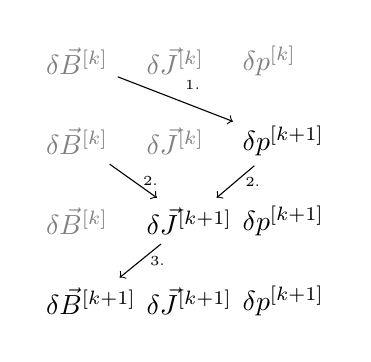
\begin{tikzpicture}[scale = 1.25, every node/.style = {shape = rectangle, anchor = west}]
  \matrix[row sep = 4mm, column sep = -1mm, ampersand replacement = \&] {
    \node[text=gray](B1) {$\delta \vec{B}^{[k]}$}; \&
    \node[text=gray](j1) {$\delta \vec{J}^{[k]}$}; \&
    \node[text=gray](p1) {$\delta p^{[k]}$}; \\
    \node[text=gray](B2) {$\delta \vec{B}^{[k]}$}; \&
    \node[text=gray](j2) {$\delta \vec{J}^{[k]}$}; \&
    \node(p2) {$\delta p^{[k+1]}$}; \\
    \node[text=gray](B3) {$\delta \vec{B}^{[k]}$}; \&
    \node(j3) {$\delta \vec{J}^{[k+1]}$}; \&
    \node(p3) {$\delta p^{[k+1]}$}; \\
    \node(B4) {$\delta \vec{B}^{[k+1]}$}; \&
    \node(j4) {$\delta \vec{J}^{[k+1]}$}; \&
    \node(p4) {$\delta p^{[k+1]}$}; \\
  };
  \draw[->] (B1) -- node [above right] {\tiny 1.} (p2);
  \draw[->] (p2) -- node [right] {\tiny 2.} (j3);
  \draw[->] (B2) -- node [right] {\tiny 2.} (j3);
  \draw[->] (j3) -- node [right] {\tiny 3.} (B4);
\end{tikzpicture}

  \caption{Individual steps within an iteration of $\hat{K}$. Grey symbols designate quantities from the previous iteration. Step 1 uses a finite difference method, outlined in \cref{sec:compute_presn}, to compute the next iteration of the pressure perturbation as an intermediary. Step 2 uses a finite volume method, discussed in \cref{sec:compute_currn}, to compute the next iteration of the current perturbation. Both are grouped together in $\hat{P}$ and solve the linearized MHD force balance. Step 3 then computes the magnetic field perturbation using the finite element method from \cref{sec:compute_Bn} to solve \textsc{Ampère}'s equation represented by $\hat{M}$, completing the cycle.}
  \label{fig:iter}
\end{figure}

For the implementation of preconditioned iterations (see \cref{sec:precon}), the cumulative approach is more convenient. To reproduce the intermediate summands, we use \cref{eq:K_partial_sum} and arrive at
\begin{gather}
  \Bpert^{(k)} = \Bpert^{[k]} - \Bpert^{[k-1]}.
\end{gather}

\subsection{Enhanced Convergence with Preconditioned Iterations}
\label{sec:precon}

Both approaches outlined in \cref{sec:iteration} hinge on the convergence of the \textsc{Neumann} series in \cref{eq:Neumann_series}. The convergence criterion for the similar geometric series of scalars is not directly applicable to operators but to their corresponding spectrum of eigenvalues. Thus we shall now consider a discretized equation of finite dimension $N$.

We start from the fixed-point relation of the previous section which has the general form
\begin{gather}
  \vec{x} = \hat{K} \vec{x} + \vec{x}_{0}. \label{eq:Arnoldi_fixed_point}
\end{gather}
$\vec{x}$ serves as a shorthand for $\Bpert$ and a reminder that the derivations in this section are not just valid for the specific problem of calculating magnetic fields. Similarly, $\vec{x}_{0}$ stands in for $\Bvac$. Assuming the linear operator $\hat{K}$ is non-singular, we can formally write down an eigendecomposition
\begin{gather}
  \hat{K} = \hat{V} \hat{\Lambda} \hat{V}^{-1},
\end{gather}
where $\hat{\Lambda}$ is a diagonal matrix with the eigenvalues,
\begin{gather}
  \hat{\Lambda} = \begin{pmatrix}
    \lambda_{1} & & & \\
    & \lambda_{2} & & \\
    & & \ddots & \\
    & & & \lambda_{N}
  \end{pmatrix} = \vec{\lambda} \hat{I},
\end{gather}
$\hat{V}$ contains the corresponding eigenvectors as its columns,
\begin{gather}
  \hat{V} = \left ( \vec{v}_{1}, \vec{v}_{2}, \dotsc, \vec{v}_{N} \right ),
\end{gather}
and $\hat{V}^{-1}$ is the inverse of $\hat{V}$. $\vec{x}$ can then be expressed in the eigenbasis with components $x_{k}'$,
\begin{gather}
  \vec{x} = \sum_{k = 1}^{N} x_{k}' \vec{v}_{k} = \hat{V} \vec{x}',
\end{gather}
and transformed back to the original basis by the inverse,
\begin{gather}
  \vec{x}' = \hat{V}^{-1} \vec{x}.
\end{gather}
Rearranging \cref{eq:Arnoldi_fixed_point} to
\begin{gather}
  \left ( \hat{I} - \hat{K} \right ) \vec{x} = \vec{x}_{0}, \label{eq:Arnoldi_direct}
\end{gather}
multiplying from the left with $\hat{V}^{-1}$ and expanding in the eigenbasis yields
\begin{gather}
  \Bigl ( \underbrace{\hat{V}^{-1} \hat{I} \hat{V}}_{\hat{I}} - \hat{\Lambda} \Bigr ) \vec{x}' = \vec{x}_{0}'.
\end{gather}
Solving for $\vec{x}'$ gives
\begin{gather}
  \vec{x}' = \left ( \hat{I} - \hat{\Lambda} \right )^{-1} \vec{x}_{0}' = \begin{pmatrix}
    \frac{1}{1 - \lambda_{1}} & & & \\
    & \frac{1}{1 - \lambda_{2}} & & \\
    & & \ddots & \\
    & & & \frac{1}{1 - \lambda_{N}}
  \end{pmatrix} \begin{pmatrix} x_{01}' \\ x_{02}' \\ \vdots \\ x_{0N}' \end{pmatrix}, \label{eq:direct_inversion}
\end{gather}
which can then be transformed back to the original basis. This approach yields a solution without resorting to series expansion and associated considerations of convergence, instead inverting the matrix directly. However, full diagonalization of $\hat{K}$ is computationally expensive, but partial diagonalization can be used to enhance convergence, or permit convergence at all, as will be seen below.

Applying the eigendecomposition to the operator series, we see that repeated application of $\hat{K}$ simplifies to
\begin{gather}
  \hat{K}^{n} \vec{x}_{0} = \underbrace{\left ( \hat{V} \hat{\Lambda} \hat{V}^{-1} \right ) \left ( \hat{V} \hat{\Lambda} \hat{V}^{-1} \right ) \dotsb \left ( \hat{V} \hat{\Lambda} \hat{V}^{-1} \right )}_{k} \vec{x}_{0}= \hat{V} \hat{\Lambda}^{n} \hat{V}^{-1} \vec{x}_{0} = \hat{V} \hat{\Lambda}^{n} \vec{x}_{0}' = \sum_{k = 1}^{N} \lambda_{k}^{n} x_{0 k}' \vec{v}_{k}.
\end{gather}
Comparing this to the solution in \cref{eq:direct_inversion}, it becomes apparent that convergence of the \textsc{Neumann} operator series is equivalent to the convergence of the geometric series of all eigenvalues. Since the geometric series only converges for $\lvert \lambda_{k} \rvert < 1$ (and only reasonably fast for $\lvert \lambda_{k} \rvert \ll 1$), we need direct inversion for the largest eigenvalues, i.e.\ partial diagonalization. To find the largest eigenvalues, we use the \textsc{Arnoldi} method summarized in \cref{app:Arnoldi}. This is a \textsc{Krylov} subspace method that reduces to the \textsc{Lanczos} method for Hermitian matrices and is also used as part of the generalized minimal residual method (GMRES). It does not involve matrix-matrix multiplication but only matrix-vector multiplication. Thus the linear operator needs not be given explicitly in matrix form, only its action on a given vector, which is fulfilled in our case for $\hat{K}$.

Using the \textsc{Arnoldi} method will give us good approximations to the largest $r$ eigenvalues, denoted as $\vec{\lambda}_{r}$ or equivalently $\hat{\Lambda}_{r}$ and commonly called \textsc{Ritz} eigenvalues, as well as an orthonormal set of associated eigenvectors, this time arranged in an $N \times r$ matrix $\hat{V}_{r}$. The latter span the \textsc{Krylov} subspace of the full eigenspace. Instead of the eigenvalue equation of full rank,
\begin{gather}
  \hat{K} \vec{v}_{k} = \lambda_{k} \vec{v}_{k} \quad \forall k = 1, 2, \dotsc, N,
\end{gather}
or equivalently,
\begin{gather}
  \hat{K} \hat{V} = \vec{\lambda} \hat{V} = \hat{V} \hat{\Lambda},
\end{gather}
we can write down the reduced eigenvalue equation in the \textsc{Krylov} subspace,
\begin{gather}
  \hat{K} \hat{V}_{r} = \vec{\lambda}_{r} \hat{V}_{r} = \hat{V}_{r} \hat{\Lambda}_{r}. \label{eq:reduced_eigvals}
\end{gather}
Note that, compared to the eigenvalue equation in full space, the $r \times r$ matrix $\hat{\Lambda}_{r}$ has to be to the right of the $N \times r$ matrix $\hat{V}_{r}$.

With the largest $r$ eigenvalues now known, we want to find a preconditioner that modifies the direct iteration step in \cref{eq:Arnoldi_fixed_point} so that the largest eigenvalues do not contribute. Usually, this is written by left-multiplying \cref{eq:Arnoldi_direct} by the inverse of a full-rank linear operator:
\begin{gather}
  \hat{\Pi}^{-1} \left ( \hat{I} - \hat{K} \right ) \vec{x} = \hat{\Pi}^{-1} \vec{x}_{0}. \label{eq:precon}
\end{gather}
We choose
\begin{gather}
  \hat{\Pi}^{-1} = \hat{I} - \hat{A}
\end{gather}
with some general matrix $\hat{A}$. \Cref{eq:precon} then becomes
\begin{gather}
  \left ( \hat{I} - \hat{A} - \left ( \hat{I} - \hat{A} \right ) \hat{K} \right ) \vec{x} = \left ( \hat{I} - \hat{A} \right ) \vec{x}_{0},
\end{gather}
which can be rearranged to resemble \cref{eq:Arnoldi_direct},
\begin{gather}
  \left ( \hat{I} - \hat{\bar{K}} \right ) \vec{x} = \bar{\vec{x}}_{0},
\end{gather}
with a modified iteration step
\begin{gather}
  \hat{\bar{K}} = \hat{A} + \left ( \hat{I} - \hat{A} \right ) \hat{K} \label{eq:Kbar}
\end{gather}
and a modified initial value
\begin{gather}
  \bar{\vec{x}}_{0} = \left ( \hat{I} - \hat{A} \right ) \vec{x}_{0}.
\end{gather}
By analogy, we can then write the explicit preconditioned iteration step as
\begin{gather}
  \bar{\vec{x}}^{[k+1]} = \hat{\bar{K}} \bar{\vec{x}}^{[k]} + \bar{\vec{x}}_{0}.
\end{gather}
Replacing the modified quantities on the right-hand side according to their definitions and rearranging gives
\begin{gather}
  \bar{\vec{x}}^{[k+1]} = \hat{A} \bar{\vec{x}}^{[k]} + \left ( \hat{I} - \hat{A} \right ) \left ( \hat{K} \bar{\vec{x}}^{[k]} + \vec{x}_{0} \right ).
\end{gather}
Now the last term in parentheses reproduces the direct, unmodified iteration yielding an unmodified $\vec{x}^{[k+1]}$,
\begin{gather}
  \bar{\vec{x}}^{[k+1]} = \hat{A} \bar{\vec{x}}^{[k]} + \left ( \hat{I} - \hat{A} \right ) \vec{x}^{[k+1]},
\end{gather}
which can again be rearranged for a final result,
\begin{gather}
  \bar{\vec{x}}^{[k+1]} = \vec{x}^{[k+1]} - \hat{A} \left ( \vec{x}^{[k+1]} - \bar{\vec{x}}^{[k]} \right ).
\end{gather}
Compared to the direct iterations, only one additional matrix-vector multiplication is necessary, but see below for details.

Now, all we need is to compute $\hat{A}$. We required that the largest $r$ eigenvalues do not contribute to iterations, so we demand
\begin{gather}
  \hat{\bar{K}} \vec{v}_{k} \overset{!}{=} \vec{0} \quad \forall k \le r.
\end{gather}
This can be compactly rewritten and expanded via \cref{eq:Kbar,eq:reduced_eigvals} to give
\begin{gather}
  \hat{\bar{K}} \hat{V}_{r} = \hat{A} \hat{V}_{r} + \left ( \hat{I} - \hat{A} \right ) \hat{K} \hat{V}_{r} = \hat{A} \hat{V}_{r} + \left ( \hat{I} - \hat{A} \right ) \hat{V}_{r} \hat{\Lambda}_{r} \overset{!}{=} \hat{0}.
\end{gather}
This can in turn be rearranged to
\begin{gather}
  \hat{A} \hat{V}_{r} \left ( \hat{\Lambda}_{r} - \hat{I} \right ) \overset{!}{=} \hat{V}_{r} \hat{\Lambda}_{r}.
\end{gather}
Right-multiplying with the inverse of $\hat{\Lambda}_{r} - \hat{I}$ yields
\begin{gather}
  \hat{A} \hat{V}_{r} \overset{!}{=} \hat{V}_{r} \hat{\Lambda}_{r} \left ( \hat{\Lambda}_{r} - \hat{I} \right )^{-1}.
\end{gather}
Now $\hat{V}_{r}$ is not square and thus cannot be inverted, but we can add a unity term on the right-hand side:
\begin{gather}
  \hat{A} \hat{V}_{r} \overset{!}{=} \hat{V}_{r} \hat{\Lambda}_{r} \left ( \hat{\Lambda}_{r} - \hat{I} \right )^{-1} \left ( \hat{V}_{r}^{\dagger} \hat{V}_{r} \right )^{-1} \hat{V}_{r}^{\dagger} \hat{V}_{r}.
\end{gather}
By direct comparison it can be seen that a solution is given by
\begin{gather}
  \hat{A} \equiv \hat{V}_{r} \hat{\Lambda}_{r} \left ( \hat{\Lambda}_{r} - \hat{I} \right )^{-1} \left ( \hat{V}_{r}^{\dagger} \hat{V}_{r} \right )^{-1} \hat{V}_{r}^{\dagger}.
\end{gather}
The inner part can be grouped to the inverse of an $r \times r$ matrix $\hat{L}_{r}$,
\begin{gather}
  \hat{L}_{r} = \hat{V}_{r}^{\dagger} \hat{V}_{r} \left ( \hat{\Lambda}_{r} - \hat{I} \right ).
\end{gather}
This can then be conveniently inverted using the LAPACK routine \texttt{zgesv} to solve for $\hat{Y}$ in
\begin{gather}
  \hat{L}_{r} \hat{Y} = \hat{I}.
\end{gather}
Since $\hat{A}$ is constant during iterations, these computations would only need to be done once before preconditioned iterations start. Note that in practice though, $\hat{A}$ is not stored explicitly, since $r \ll N$ -- in test runs, $r \approx \num{1e1}, N \approx \num{1e5}$. Instead of keeping $N^2$ entries of the dense matrix $\hat{A}$ in storage, we keep $N r$ entries of $\hat{V}_{r}$ and $r^2$ entries of $\hat{\Lambda}_{r} \hat{L}_{r}^{-1}$. Applying the matrices on a given $\vec{x}$ from right to left then requires additional matrix-vector multiplications, but in the worst case, this involves only $2 N r + r^2$ floating-point operations compared to $N^2$ for one matrix-vector multiplication with full $\hat{A}$. For an overview on matrix sizes, see \cref{tab:matrix_dimensions}.
\begin{longtable}{ll}
  \caption{Dimensions of quantities used in derivation of preconditioned iterations.}
  \label{tab:matrix_dimensions} \\
  \toprule
  Quantity & Dimension \\
  \midrule
  \endfirsthead
  \toprule
  Quantity & Dimension \\
  \midrule
  \endhead
  $\vec{x}$ & $N$ \\
  $\vec{\lambda}_{r}$ & $r$ \\
  $\vec{v}_{k}$ & $N$ \\
  $\hat{\Lambda}_{r}$ & $r \times r$ \\
  $\hat{V}_{r}$ & $N \times r$ \\
  $\hat{V}_{r}^{\dagger}$ & $r \times N$ \\
  $\hat{A}$ & $N \times N$ \\
  $\hat{L}_{r}$ & $r \times r$ \\
  \bottomrule
\end{longtable}
It should be noted that the approximation error of the \textsc{Ritz} eigenvalues relative to the true eigenvalues decreases with the size of the \textsc{Krylov} subspace. This means that more \textsc{Arnoldi} iterations should be completed than is purely necessary for the expected number of eigenvalues with absolute value below a given threshold. Even if most of them are not used in the preconditioner, without sufficient accurcy in the largest eigenvalues the preconditioner will fail to assure convergence. As a rule of thumb, there should be \numrange{2}{3} times as many \textsc{Arnoldi} iterations as there are \textsc{Ritz} eigenvalues used with the preconditioner.

%%% Local Variables: 
%%% mode: latex
%%% TeX-master: "../magdif"
%%% End: 
